\chapter{Transparent alignment in Kotlin}\label{chapter:alignment}
The alignment, discussed in Section \ref{subsection:alignment}, is a crucial feature that is necessary to provide in order to create a working implementation of the \textbf{Aggregate programming} paradigm. 

The first step for finding a solution of a problem is to define a simple use case, which is going to be the base of the resolution attempts. A good starting point is code in Listing \ref{code:first_alignment_code_example}, which was also discussed previously in Section \ref{subsection:alignment}. In order to be coherent with the final solution, the code is now written in Kotlin and the nbr-expression is now called \textit{neighboring}.
\begin{lstlisting}[caption={Starting point code to resolve the alignment problem}, captionpos=b, language=Kotlin, label={code:first_alignment_code_example}]
fun f1() {neighboring(e1)}
fun f2() {neighboring(e1)}
        
f1()
f2()
\end{lstlisting}
The goal that needs to be achieved is to find an alignment solution that is able to keep track of the current computational state of a device, making it possible to align only the correct expressions with each other. In this example, it is necessary to find a unique way to identify the execution of the neighboring expression in the body of the \textit{f1} function from the one in the \textit{f2} function.\newline
It is not considered right now the computing device identification, since it is not a core problem in these attempts. Once the base case is solved, then further complexities of the alignment problem are going to be analyzed, such as the branch construct.

There are key aspects that are considered for this study and that are used to compare the different approaches:
\begin{itemize}
    \item \textbf{Availability for Kotlin multiplatform}: it is important to keep in mind that DSL is developed by using Kotlin multiplatform, which choice is discussed in Section \ref{section:technology_choices}. The approaches chosen must be available for a Kotlin multiplatform architecture;
    \item \textbf{Portability}: the alignment solution has to work for all the targeted platforms by Kotlin Multiplatform, which are Native, JavaScript and JVM. Multiple device computing on the same platform have to be able to align correctly;
    \item \textbf{Interoperability}: the solution should allow devices executing on different platform to align;
    \item \textbf{Efficiency}: one aspect to consider is the efficiency, because it can not be produced an elaborated solution that needs devices with high computational requirements;
    \item \textbf{Transparency}: finally, this feature has to be transparent to the final user, without making the developer write ulterior code to make the alignment work.
\end{itemize}

Different approaches have been tried to find a solution, and, for each attempt they are discussed the advantages and the disadvanteges. The following sections analyze all the possibilities taken in consideration: Section \ref{section:stacktraces_hashes} goes into details of the attempts with stacktraces and hashes, Section \ref{section:annotation_ksp} exploit the problem with annotations and KSP, understanding their limits. Finally, Section \ref{section:compiler_plugin_solution} describes in details the solution adopted, by developing a Kotlin compiler plugin. In each section there is a table that recaps the characteristics for each technology tried for the alignment based on the key aspects highlighted previously.

\section{Stacktraces and hashes}\label{section:stacktraces_hashes}
Since the alignment problem is quite complex, the firsts attempts regards simple strategies without the concern of efficiency, trying to use already existing Kotlin functionalities to generate a unique identifier.

One way of keeping track of the functions called during a program execution is by checking the \textbf{stacktrace}. This leads to one of the possible solutions, which is throwing exceptions whenever an aggregate programming construct is computed, and then using the generated exception stacktrace as identifier.\newline
The stacktraces can be generated in all the platforms that the DSL aims to target. On each platform, the stacktrace is identical for every program execution, meaning that it is possible to align different devices that are executing the same program on the same target.\newline
Moreover, this solution offers transparency to the final user, because the alignment can work without having the developer to write additional code.\newline
On the other hand, this option presents two main problems that can not be avoided:
\begin{enumerate}
    \item The first problem regards the efficiency of this solution. Since an aggregate program runs continuously on each computing device, an enormous amount of exception would be thrown, causing delays that in a distributed system can cause issues;
    \item The second problem refers to the interoperability of device computing on different targeted platforms. The stacktraces generated by the Native target are completely different from the one generated by JavaScript and JVM, and they represent information in a non-identical way. This means that devices running on different platforms can not align correctly, since the identifier generated for the sequence of the functions called does not match.
\end{enumerate}

Following a similar line of reasoning, the next attempt involved the \textbf{hash-codes}. Kotlin provides a method that given an object returns its hash-code, and it is guaranteed that the hash-code generated is always the same whenever two objects are equal to each other. In order to take advantage of this feature, it was created a new class called \textit{Event}, which has the role to encapsulate the DSL expression that was currently being computed by a device, and then use the object hash-code as identifier. In general, this is not a suitable solution: the hash generated is the same during a single execution, but it is not when running multiple devices that have to communicate, meaning that the alignment can not be achieved, since the identifiers can be different even though they should not be.\newline
This issue is present also when trying to align devices running on different platforms, but there is an additional problem: the hash-code generated from a target is not the same in another target, creating a discrepancy impossible to overcome.

\begin{table}[!ht]
    \small
    \centering
    \begin{tabular}{|l|c|c|c|c|c|}
    \hline
    \textbf{} &
      \begin{tabular}[c]{@{}c@{}}Available for\\ Kotlin \\ Multiplatform\end{tabular} &
      \begin{tabular}[c]{@{}c@{}}Allows\\ same target\\ interoperability\end{tabular} &
      \begin{tabular}[c]{@{}c@{}}Allows\\ different targets\\ interoperability\end{tabular} &
      \multicolumn{1}{l|}{\begin{tabular}[c]{@{}l@{}}Acceptable\\ efficiency\end{tabular}} &
      \begin{tabular}[c]{@{}c@{}}Transparent\\ to the\\ final user\end{tabular} \\ \hline
    \textbf{Stacktrace} &
      yes &
      yes &
      no &
      no &
      yes \\ \hline
    \textbf{Hash} &
      yes &
      no &
      no &
      yes &
      yes \\ \hline
    \end{tabular}
    \caption{Comparison between stacktrace and hash for solving the alignment problem}
    \label{tab:stacktrace_hash_table}
\end{table}

Considering these attempts and their characteristics, it is possible to conclude that they are not suitable as resolution of the alignment problem. In order to give a clear view of their pros and cons, the characteristics of the alternative just discussed are recapped in Table \ref{tab:stacktrace_hash_table}.

\section{Annotations and KSP}\label{section:annotation_ksp}
Since simple Kotlin functionalities are not feasible for solving the alignment problem, another possibility is to try different metaprogramming alternative, such as the ones discussed in Chapter \ref{chapter:metaprogramming}.

The first metaprogramming technique taken in consideration is \textbf{annotations}. As explained in Section \ref{section:annotation}, annotations can be used to attach additional metadata to elements in the code, which can be used to create specific behaviors. For example, it is possible to use them to define that a function should be causing the alignment and specify through the annotations how to handle it.\newline
Before diving in the technical details of how the alignment could be performed, a few considerations must be made:
\begin{itemize}
    \item A key aspect of this project is the interoperability, achieved by using Kotlin multiplatform, and the chosen targets are Native, JavaScript and JVM. While this thesis is being redacted, Kotlin\textbackslash JS does not support annotations, creating a compatibility issue that is difficult to overcome;
    \item In order to take advantage of the metadata provided by annotations, the developer should annotate manually every element in the source code whenever the alignment is required. This is not acceptable, since a requirement of the solution is the transparency for the final user.
\end{itemize}

The next alternative that involves metaprogramming is \textbf{KSP} (Kotlin Symbol Processing), which is described in details in Section \ref{section:ksp}. Starting from KSP 1.0.1, it is possible to use KSP on multiplatform projects \cite{ksp_multiplatform}, which includes also the targets necessary to reach successfully the outcome desired.\newline
KSP allows the creating of lightweight compilers, providing an API that hides all the complexities that a complete compiler plugin would involve. While designing a possible solution, it is necessary to keep in mind the biggest limitation that this technology brings within, which is the impossibility to modify the source code.\newline
Since KSP can access the code at compile time, it can be used to extract information that can be used to build a custom stacktrace that keeps track of the sequence of functions called. Then, this custom stack can be used as identifier when needed. For this reason, it has been created a class \textit{Stack}, which interface is in Listing \ref{code:stack_interface_ksp}.
\begin{lstlisting}[caption={Stack interface for KSP}, captionpos=b, language=Kotlin, label={code:stack_interface_ksp}]
interface Stack {
    fun currentPath(): String
    fun align(token: String): Unit
}
\end{lstlisting}
By using the \textit{Stack} it is possible to add to a data structure everything necessary for the alignment, which might be for example function calls. Considering the base case cited previously in Listing \ref{code:first_alignment_code_example}, when executing \textit{f1}, the stack list should contain \textit{[f1, neighboring]}, and when computing \textit{f2} would be \textit{[f2, neighboring]}, making it possible to uniquely identify the two different expressions.\newline
Trying to obtain the result just described, the problem can be divided in two smaller steps:
\begin{enumerate}
    \item The aggregate programming constructs are part of the DSL functions exposed to the final user, meaning that it is not possible for the user to change their implementation in any way while using it. Moreover, the name of these functions is known in advanced. This leads to create a simple solution for handling them, which consists on changing their implementations and adding a line of code that it is responsible to insert in the \textit{Stack} data structure the function name. For example, in the \textit{neighboring} implementation there is a function call to align that add its name to the stack.
    \item The second problem, which is more complex, can not be solved in the same way, since it would be the final user to manually solve the alignment problem. The solution would be to modify the functions \textit{f1} and \textit{f2} using KSP and adding the same line of code discussed for the previous case. On the other hand, the direct modification of the source code is not allowed by KSP, which means that the only solution would be to recreate the same code of the user, with the added function calls. This solution would be feasible for simple use cases, but it is not efficient when dealing with complex systems.
\end{enumerate}
This leads to the conclusion that it is crucial for the solution of the alignment problem the possibility to modify the source code. KSP can be used as a temporary solution for some use cases, also taking advantage of the simple and powerful API that it provides, but the downsides are important factors to consider.

\begin{table}[!ht]
    \small
    \centering
    \begin{tabular}{|l|c|c|c|c|c|}
    \hline
    \textbf{} &
      \begin{tabular}[c]{@{}c@{}}Available for\\ Kotlin \\ Multiplatform\end{tabular} &
      \begin{tabular}[c]{@{}c@{}}Allows\\ same target\\ interoperability\end{tabular} &
      \begin{tabular}[c]{@{}c@{}}Allows\\ different targets\\ interoperability\end{tabular} &
      \multicolumn{1}{l|}{\begin{tabular}[c]{@{}l@{}}Acceptable\\ efficiency\end{tabular}} &
      \begin{tabular}[c]{@{}c@{}}Transparent\\ to the\\ final user\end{tabular} \\ \hline
    \textbf{Stacktrace} & yes & yes                   & no                    & no  & yes \\ \hline
    \textbf{Hash}       & yes & no                    & no                    & yes & yes \\ \hline
    \textbf{Annotation} & no  & yes (manually)        & yes (manually)        & yes & no  \\ \hline
    \textbf{KSP}        & yes & yes                   & yes                   & no  & yes \\ \hline
    \end{tabular}
    \caption{Comparison between stacktrace, hash, annotation and KSP for solving the alignment problem}
    \label{tab:annotation_ksp_table}
\end{table}

Concluding, the characteristics of annotation and KSP are added in Table \ref{tab:annotation_ksp_table} alongside with the stacktrace and hash ones, summarizing the considerations made on all the alternatives considered up until this point.

\section{KCP: solution with total transparency and portability}\label{section:compiler_plugin_solution}
\textbf{Kotlin compiler plugins} are another metaprogramming alternative. As discussed previously in Section \ref{section:compiler_plugin_explanation}, the development of a compiler plugin requires a lot of time and study, but they also provide a total freedom when trying to modify the code at compile time.

The following considerations prove that a plugin can be used to solve the alignment problem:
\begin{itemize}
    \item When developing project using Kotlin multiplatform, under the hood the compiler translate the Kotlin code into the code of the targets. Before doing that, it is transformed into an \textit{Intermediate Representation}, called \textbf{IR}, which as been discussed in Section \ref{section:kotlin_ir}. This representation allows the creation of multiplatform compiler plugins, without the need to distinguish the plugin between the different platforms;
    \item Since the source code is completely available at compile time, it is possible to analyze it in order to make the plugin understand when the alignment is needed. Then, new code can be generated to guarantee the correct alignment, which can be similar to the stack discussed for KSP. Moreover, since the generation is based on the intermediate representation, this allows the interoperability between the different project targets;
    \item Finally, the plugin modifications are applied at compile time, which does not impact in a relevant way the execution time. The code generation is also totally transparent to the user, that does not have to worry about the alignment.
\end{itemize}

The Kotlin compiler plugin solution is the chosen one for creating this crucial feature, because, comparing it with the other alternatives, it is the one that respects all the requirements. All the characteristics of the analyzed possibilities are summarized in Table \ref{tab:kcp_table}.
\begin{table}[!ht]
    \small
    \centering
    \begin{tabular}{|l|c|c|c|c|c|}
    \hline
    \textbf{} &
      \begin{tabular}[c]{@{}c@{}}Available for\\ Kotlin \\ Multiplatform\end{tabular} &
      \begin{tabular}[c]{@{}c@{}}Allows\\ same target\\ interoperability\end{tabular} &
      \begin{tabular}[c]{@{}c@{}}Allows\\ different targets\\ interoperability\end{tabular} &
      \multicolumn{1}{l|}{\begin{tabular}[c]{@{}l@{}}Acceptable\\ efficiency\end{tabular}} &
      \begin{tabular}[c]{@{}c@{}}Transparent\\ to the\\ final user\end{tabular} \\ \hline
    \textbf{Stacktrace} & yes & yes                   & no                    & no  & yes \\ \hline
    \textbf{Hash}       & yes & no                    & no                    & yes & yes \\ \hline
    \textbf{Annotation} & no  & yes (manually)        & yes (manually)        & yes & no  \\ \hline
    \textbf{KSP}        & yes & yes                   & yes                   & no  & yes \\ \hline
    \textbf{KCP}        & yes & yes                   & yes                   & yes & yes \\ \hline
    \end{tabular}
    \caption{Comparison between stacktrace, hash, annotation, KSP and Kotlin compiler plugin for solving the alignment problem}
    \label{tab:kcp_table}
\end{table}

The chosen approach is similar to the one discussed for KSP in Section \ref{section:annotation_ksp}: the best way to understand if two different devices are aligned is by using a custom stack, which can keep track of the sequence of functions called during the computation. In order to do so, the stack is used to push the function name into the data structure when a function is called, and then it is popped when the control flow exits that function. A similar behavior is provided in the case of the domain restriction caused by the branch construct, pushing in the stack the condition evaluated.

This important data structure has been called \textbf{Stack} and its interface is shown in Listing \ref{code:stack_interface_compiler_plugin}.
\begin{lstlisting}[caption={Stack interface for Kotlin compiler plugin solution}, captionpos=b, language=Kotlin, label={code:stack_interface_compiler_plugin}]
interface Stack<X> {
    fun currentPath(): Path
    fun alignRaw(token: X?): Unit
    fun dealign(): Unit
}
\end{lstlisting}
The stack has an internal mutable list that is updated when calling the method \textit{alignRaw} and \textit{dealign}. Specifically, \textit{alignRaw} is used to push a generic identifier into the stack, \textit{dealign} is used to pop it.\newline
When a device needs to know its computational state, it can retrieve its path using the function \textit{currentPath}. A \textbf{Path} is a data class that is used as a wrapper of the current stack state, in order to return the immutable list, following Kotlin best practice. Its implementation is in Listing \ref{code:path_compiler_plugin}.
\begin{lstlisting}[caption={Path dataclass for Kotlin compiler plugin solution}, captionpos=b, language=Kotlin, label={code:path_compiler_plugin}]
data class Path(val path: List<Any?>)
\end{lstlisting}

The data structures that can be used to store the information about the computation has been defined, which lays the foundations of the alignment solution. It is now necessary to provide a method that actually update the stack correctly, without having to do it manually. This is also going to be the function call generated by the compiler plugin to perform the alignment.
\begin{lstlisting}[caption={Stack interface for KSP}, captionpos=b, language=Kotlin, label={code:alignedOn_compiler_plugin}]
fun <R> alignedOn(pivot: Any?, body: () -> R): R {
    stack.alignRaw(pivot)
    return body().also { stack.dealign() }
}
\end{lstlisting}
The method \textit{alignedOn} in Listing \ref{code:alignedOn_compiler_plugin} needs to be explained further, since its behavior is central in the solution proposed.\newline
The function signature accepts two parameters: the first one is the \textit{pivot}, which is the identifier that is going to be pushed in the stack, the second one is \textit{body}, which is the element that is going to be computed. For example, considering the base example reported at the beginning of this chapter in Listing \ref{code:first_alignment_code_example} and supposing the computation of \textit{f1}, the \textit{pivot} would be the name of the function, that is the string \textit{f1}, and the body would be \textit{f1()}, which performs the computation of that function.\newline
The implementation of \textit{alignedOn} is entitled update the stack pushing the pivot, then it executes the function taken as parameter and returns as output the value computed. Once the computation of the function is completed, it also resets the stack at its previous state.

The basic information to explain the solution has been presented, and it is now necessary to divide the problem in two smaller steps. In Section \ref{subsection:function_alignment} it is going to be discussed how to perform the alignment when dealign with function calls, giving also example of the generation of the code created by the compiler plugin. Then, in Section \ref{subsection:branch_alignment} it is going to be explained how to guarantee the alignment when there are branches that cause domain restriction.

\subsection{Function alignment with KCP}\label{subsection:function_alignment}
Before describing how to generate code using the compiler plugin, it is necessary to define what Kotlin compiler plugin should generate in the context of functions.

Listing \ref{code:generation_first_alignment_code_example} shows how Listing \ref{code:first_alignment_code_example} is modified during compilation by the compiler plugin.
\begin{lstlisting}[caption={Generation goal to handle the alignment of Listing \ref{code:first_alignment_code_example}}, captionpos=b, language=Kotlin, label={code:generation_first_alignment_code_example}]
fun f1() {
    alignedOn("neighboring"){
        neighboring(e1)
    }
}
fun f2() {
    alignedOn("neighboring"){
        neighboring(e1)
    }
}
            
alignedOn("f1"){
    f1()
}
alignedOn("f2"){
    f2()
}
\end{lstlisting}
To each function call now corresponds a new call to \textit{alignedOn} function, creating the mechanism of alignment.\newline
While executing the code in Listing \ref{code:generation_first_alignment_code_example}, this is what happen to the stack:
\begin{itemize}
    \item First, the \textit{alignedOn} on line 12 is executed and the state of the stack is now \textit{[f1]};
    \item Then, \textit{f1} is computed, which causes another \textit{alignedOn} call. The stack is updated, and its current value is now \textit{[f1, neighboring]};
    \item While executing the neighboring function, the device looks into the messages received by its neighbors in order to find fields that match the current stack value \textit{[f1, neighboring]}. Those neighbors are the one aligned with the considered computing device;
    \item Then the \textit{alignedOn} call at line 2 has completed its execution, so there is another update on the stack, which dealign from the current state. The stack is \textit{[f1]};
    \item Also the \textit{alignedOn} on line 12 is finished, causing the stack to be empty again;
    \item The exact behavior happens when computing \textit{f2}, with the difference that the stack when computing the neighboring function is \textit{[f2, neighboring]}. In this way, only the neighbors values found that executed \textit{f2} and then \textit{neighboring} are considered.
\end{itemize}

Now that the end result that wants to be achieved for this base case is clear, the compiler plugin can be explained in details. Since most of a basic plugin implementation has been explained in the example in Section \ref{section:compiler_plugin_example}, only the crucial part of the transformation of the code are going to be discussed.

The \textbf{IrGenerationExtension}, before registering the transformer necessary to perform the code modification, needs to retrieve two elements, which absence would preclude the execution of the plugin. The user would be informed with a console message in the case that, during the compilation, the required elements were not found.\newline
The referred elements are:
\begin{enumerate}
    \item \textbf{The alignedOn function declaration}: in order to be able to call an already existent function, it is necessary to specify to the compiler to look for that function. In this case it is necessary the reference to \textit{alignedOn}, discussed in Listing \ref{code:alignedOn_compiler_plugin};
    \item \textbf{The aggregate context}: the functions exposed by the DSL are encapsulated in the \textbf{AggregateContext} class, which also contains the reference to the stack instance. Since it is possible to modify the stack only through its instance, the aggregate context class retrieved here can be used to get the instance of the object when calling the \textit{alignedOn} function. More details about the \textit{AggregateContext} class are going to be given in Chapter \ref{chapter:collektive}.
\end{enumerate}

In order to provide some optimization, not every element of the source code is going to be modified by the compiler plugin, but only the necessary ones. If the final user needs a particular alignment not covered by the developed plugin, he can use the \textit{alignedOn} function manually.\newline
The entry point of the DSL is the function \textbf{aggregate}, which takes as parameter a function type with receiver. The receiver is the \textit{AggregateContext}, meaning that all the call members of the receiver can be used inside the \textit{aggregate} function call.\newline
After retrieving the necessary elements, the \textit{IrGenerationExtension} registers the \textbf{AggregateCallTransformer}, which visits through the visitor pattern all the function calls looking for all the \textit{aggregate} call. Thanks to that, to compiler plugin knows that inside that function calls there might be the necessity to modify the code to provide the alignment feature.

For each aggregate function call the transformation is then delegated to the \textbf{AlignmentTransformer}, which handles the alignment required by the function calls and the branch constructs.\newline
Starting from the function calls, this is what happen:
\begin{itemize}
    \item The \textit{visitCall} provided by the transformer's interface is overridden, providing access to all the children of the aggregate function call that are also calls;
    \item Then the behavior can be divided in three different cases:
    \begin{enumerate}
        \item If the function call has been already aligned, any modification is applied to the code;
        \item Otherwise, in order to provide another optimization, it is checked if the considered function call or any of its children has a reference to the \textit{AggregateContext}. Only the function of the DSL, which are \textbf{neighboring}, \textbf{repeating} and \textbf{sharing} have a reference to that context. This means that everything not related to the DSL does not require to be modified for the alignment problem. This research is performed by checking the current function call's receivers and by the \textbf{AggregateRefChildrenVisitor} whenever it is necessary to visit the children.\newline
        If any of the elements analyzed have a reference to the \textit{AggregateContext}, then the code is not transformed;
        \item If the \textit{AggregateContext} reference is found, then the transformation proceeds. 
    \end{enumerate}
    Of the three possible outcomes, only the third one makes the computation continue, in all the other cases the not modified function call is returned. For this reason, it is necessary to assume that an \textit{AggregateContext} reference has been found in order to continue to explain how the transformation works;
    \item In order to be able to create a new function call in the source code, it has to be declared inside an \textbf{irStatement}, which is used to define also the scope where the function is created;
    \item Inside the \textit{irStatement} is then created the \textit{alignedOn} function call.
    \item Finally, the transformed function call is returned.
\end{itemize}

The creation of the \textit{alignedOn} function call is crucial for this transformation, and it is going to be described in more details.\newline 
Once created the \textit{irStatement} it is possible to create a new \textbf{irCall} like shown in Listing \ref{code:aligned_on_creation}.
\begin{lstlisting}[caption={Generation goal to handle the alignment of Listing \ref{code:first_alignment_code_example}}, captionpos=b, language=Kotlin, label={code:aligned_on_creation}]
irCall(alignedOnFunction).apply {
    // Set generics type
    putTypeArgument(expression.type)
    // Set aggregate context
    putArgument(
        alignedOnFunction.dispatchReceiverParameter!!,
        aggregateContextReference
    )
    // Set the argument that is going to be pushed in the stack
    putValueArgument(
        irString(
            expression.symbol.owner.kotlinFqName.asString()
        )
    )
    // Create the lambda that is going to call expression
    val lambda = buildLambdaArgument(
        pluginContext,
        aggregateLambdaBody,
        expression
    )
    putValueArgument(1, lambda)
}
\end{lstlisting}
The \textit{irCall} builds a new \textit{alignedOnFunction}, which is the reference to the \textit{alignedOn} function responsible for the alignment. It is set the type argument and the dispatch receiver, which are both necessary to create a correct element. Then, the value argument is the first parameter of the \textit{alignedOn} function, and it is created using the name of the originating expression. Finally, the second value argument is the body of the call of the original function, which is recreated as a lambda.\newline
The lambda as argument is created in another function, which is implemented as follows:
\begin{lstlisting}[caption={Generation goal to handle the alignment of Listing \ref{code:first_alignment_code_example}}, captionpos=b, language=Kotlin, label={code:lambda_creation}]
pluginContext.irFactory.buildFun {
    name = Name.special("<anonymous>")
    this.returnType = expression.type
    this.origin = IrDeclarationOrigin.LOCAL_FUNCTION_FOR_LAMBDA
    this.visibility = DescriptorVisibilities.LOCAL
}.apply {
    this.patchDeclarationParents(this@buildLambda.parent)
    if (expression.symbol.owner.returnType.isUnit()) {
        this.body = context.
                        irBuiltIns.
                        createIrBuilder(symbol).
                        irBlockBody {+expression}
    } else {
        this.body = context.
                        irBuiltIns.
                        createIrBuilder(symbol).
                        irBlockBody {+irReturn(expression)}
    }
}
\end{lstlisting}
From line 2 to 5 of Listing \ref{code:lambda_creation} standard parameters are set, such as the return type, the lambda parent and information that inform the compiler that it is dealing with an anonymous function. Then, if the original expression return type is unit, then the body of the lambda is just the expression itself. Otherwise, a return block is added, which contains the original function call.

To recap the process it is possible to start from the simple code in Listing \ref{code:base_for_transformation_example}.
\begin{lstlisting}[caption={Generation goal to handle the alignment of Listing \ref{code:first_alignment_code_example}}, captionpos=b, language=Kotlin, label={code:base_for_transformation_example}]
aggregate {
    println("do not align")
    fun calculate() {
        neighboring("test")
    }
}
\end{lstlisting}
The Figure \ref{fig:ir_trasformation_with_code_elements} shows how the various elements developed for the compiler plugin work together.
\begin{figure}[!ht]
    \centering
    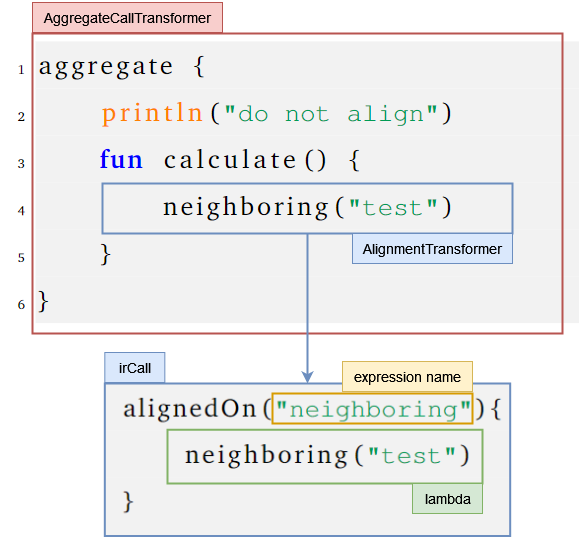
\includegraphics[scale=0.65]{document/chapters/3-alignment/images/ir_trasformation_with_code_elements.png}
    \caption{The Kotlin compiler plugin architecture \cite{compiler_plugins_jetbrains}}
    \label{fig:ir_trasformation_with_code_elements}
\end{figure}
The \textit{AggregateCallTransformer} finds the aggregate call, the \textit{AlignmentTransformer} is able to understand which function needs to be aligned, which in this example is \textit{neighboring}. Then the new function call is created, with the two parameters: the name of the original function and its call.

\subsection{Branch construct alignment}\label{subsection:branch_alignment}
As anticipated in Section \ref{subsection:alignment}, also the branch construct creates a domain restriction that needs to be handled by the alignment feature.\newline
Again, it is necessary to define the required result that has to be achieved by the compiler plugin.
\begin{lstlisting}[caption={Generation goal to handle the alignment of Listing \ref{code:first_alignment_code_example}}, captionpos=b, language=Kotlin, label={code:branches_alignment_code_example}]
val number = (0..10).random()
if (number > 5) {
    neighboring("higher")
} else {
    neighboring("lower")
}
\end{lstlisting}
Given the example in Listing \ref{code:branches_alignment_code_example} its transformation would be the one reported in Listing \ref{code:generation_branches_alignment_code_example}.
\begin{lstlisting}[caption={Generation goal to handle the alignment of Listing \ref{code:first_alignment_code_example}}, captionpos=b, language=Kotlin, label={code:generation_branches_alignment_code_example}]
val number = (0..10).random()
if (number > 5) {
    alignedOn("[number > 5, true]"){
        alignedOn(neighboring){
            neighboring("higher")
        }
    }
} else {
    alignedOn("[constant, false]"){
        alignedOn(neighboring){
            neighboring("lower")
        }
    }
}
\end{lstlisting}
The \textit{alignedOn} function calls at line 4 and 10 are created by the mechanism explained previously is Section \ref{subsection:function_alignment}, and at line 3 and 9 there are the alignment functions for the branches.\newline
Supposing that the random generated number is 7, the stack during the computation of the code in Listing \ref{code:generation_branches_alignment_code_example} is the following:
\begin{enumerate}
    \item Since the value of number is 7, the condition of the \textit{if} at line 2 is true and its body is executed;
    \item The alignment function at line 3 allows putting in the stack \textit{[[number > 5, true]]}, which is a pair of the condition evaluated and its actual value, which is true;
    \item Then, to the stack it is added the neighboring call, leading to \textit{[[number > 5, true], neighboring]}. This means that the neighboring function align only whenever the condition of the \textit{if} is true, meaning that it is higher than 5;
    \item After the computation of neighboring, it is popped from the stack, leaving again only \textit{[[number > 5, true]]};
    \item Finally, the body of the \textit{if} has been successfully executed and the stack can be cleared.
\end{enumerate}

Before diving into the creation of the \textit{alignedOn} parameters, it is necessary to understand how the IR syntax tree handled the branches when there are multiple conditions, which is slightly different from the single condition just presented. Kotlin IR works with binary trees, which means that when it has to handle branches with multiple conditions, it creates nested branches.\newline
For example, considering Listing \ref{code:multiple_branches_example}, it is represented as shown in Figure \ref{fig:multiple_branches_ir_example}.
\begin{lstlisting}[caption={Example of code where a branch has multiple conditions}, captionpos=b, language=Kotlin, label={code:multiple_branches_example}]
if (a && b) {
    function()
}
\end{lstlisting}

\begin{figure}[!ht]
    \centering
    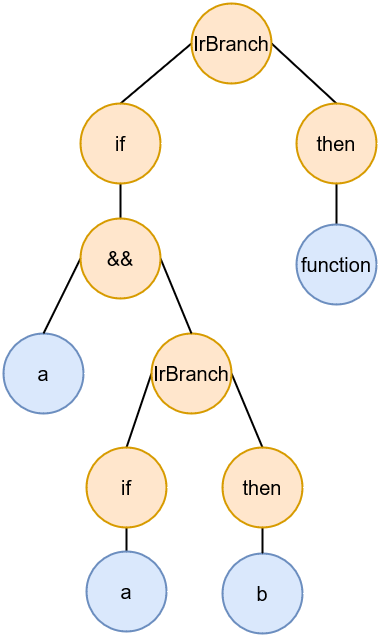
\includegraphics[scale=0.55]{document/chapters/3-alignment/images/ir_representation_branches.png}
    \caption{The IR of a branch with multiple condition shown in Listing \ref{code:multiple_branches_example}}
    \label{fig:multiple_branches_ir_example}
\end{figure}
The Figure \ref{fig:multiple_branches_ir_example} shows that a branch is handle like follows:
\begin{itemize}
    \item The first branch of the if evaluates the condition \textit{a};
    \item If \textit{a} is true, then it is evaluated the condition \textit{b}. This creates the chance to align \textit{b} based on the evaluation of \textit{a}, because after the evaluation of \textit{a} the stack is \textit{[[a,true]]}, which means that \textit{b} align only with the neighbors that evaluated \textit{a} as true;
    \item After obtaining both the result of \textit{a} and \textit{b}, it is calculated the value of \textit{a \&\& b};
    \item If the full condition is evaluated as true, the stack is \textit{[a \&\& b, true]};
    \item Then it is computed \textit{function()}, which is aligned based on the stack just created.
\end{itemize}

It is the \textbf{AlignmentTransformer} that, as well as the functions' alignment, handles the branches. It overrides two different functions:
\begin{itemize}
    \item \textbf{visitBranch}: it represents the \textit{if} and the \textit{else if} condition;
    \item \textbf{visitElseBranch}: it is used for the \textit{else} branch;
\end{itemize}
The way these two types of elements are handled is the same, so just the normal \textit{if} branch is discussed.

The result of a branch is divided in the IR in blocks or expressions:
\begin{itemize}
    \item \textbf{IrBlock}: in this case the \textit{if} result consists of a block, like this:
\begin{lstlisting}
if(condition){
    function()
    function()
}
\end{lstlisting} 
    \item \textbf{IrExpression}: the result of the \textit{if} it is not encapsulated in brackets, it is composed by one expression:
\begin{lstlisting}
if(condition) function()
\end{lstlisting}
\end{itemize}

The way the \textit{IrBlock} and the \textit{IrExpression} requires a slightly different implementation: if a branch was constituted by an \textit{IrBlock}, when creating the \textit{alignedOn} function call it is necessary to keep in mind that the second parameter is going to be a block and not a single expression.\newline
The building of the \textit{alignedOn} function call is the same of the code shown in Listing \ref{code:lambda_creation}, the only difference is the creation of the parameters. 

The first parameter is the name of the element that is going to be put in the stack. As seen before, just the name of the condition is not sufficient, since the alignment is based on the name and the condition value. For this reason, the first parameter is a pair constituted by the condition name and its value, like this: \textit{[condition, true]}.\newline
When the condition is a variable, a function call or an anonymous function, the stack will contain the exact name of the element. In the case of a constant, for example just the value \textit{true}, then it is used the placeholder \textit{constant}.

The second parameter is constituted by a lambda that contains the body of the \textit{if}. Since it is considered in this discussion that the body is an \textit{IrBlock}, then it is necessary to create a new block that is going to create the lambda.
\begin{lstlisting}[caption={Creation of the lambda body when modifying a \textit{IrBranch}}, captionpos=b, language=Kotlin, label={code:ir_block_branch_example}]
this.returnType = getReturnType(lastExpression)
this.body = context.
            irBuiltIns.
            createIrBuilder(symbol).
            irBlockBody {
                for (bodyStatement in expression.statements) { 
                    +bodyStatement 
                }
                +irReturn(lastExpression)
            }
\end{lstlisting}
There are three main things need to be done when creating the lambda body, and they are shown in Listing \ref{code:ir_block_branch_example}:
\begin{enumerate}
    \item \textbf{Setting the return type}: since the body of the \textit{if} is a block, it is constituted by multiple expression. The last expression return type defines the return type of the block. In order to be able to get the result of the \textit{if} construct, it is necessary to set it correctly;
    \item \textbf{Creating the IrBlock}: the block created contains all the expressions of the previous block but the last one. In this way, the behavior of the block is not going to change;
    \item \textbf{Setting the return type}: finally, the last element to add to the block is the return, which is defined by the last expression. It must be created inside the \textit{irReturn} element, which is used to create a special block that is expected to match the return type.
\end{enumerate}

This constituted the whole behavior of the compiler plugin when dealing with a \textit{IrBranch}, but the transformation is similar when dealing with an \textit{IrElseBranch}.\newline
One final details of the transformation of the branches is in common with the function handling: the alignment is required if and only if there are aggregate programming construct calls, which means that modifying a block of an \textit{IrBranch} when its body does not involve any aggregate function it is useless. For this reason, the same control performed for the function calls is performed here, which means that, when visiting any branch, only if the \textit{AggregateContext} reference is found in any of it body expression or expressions' children, then the alignment transformation is actuated. This enhances the performances of the Kotlin compiler plugin created.
